\titleformat{\chapter}[display]
  {\normalfont\bfseries}{}{0pt}{\Large}


\chapter{Annexes}

\begin{figure}[ht]
\centering
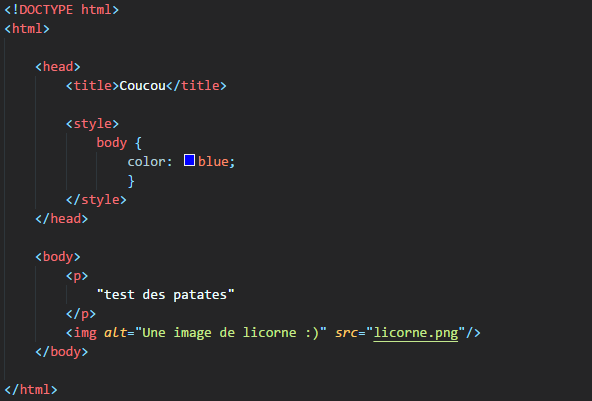
\includegraphics[height=0.8\textwidth]{html1.png}
\caption{\label{fig:html1}Fichier HTML de base sur lesquelles ont été réalisé les tests}
\end{figure}

\begin{figure}[ht]
\centering
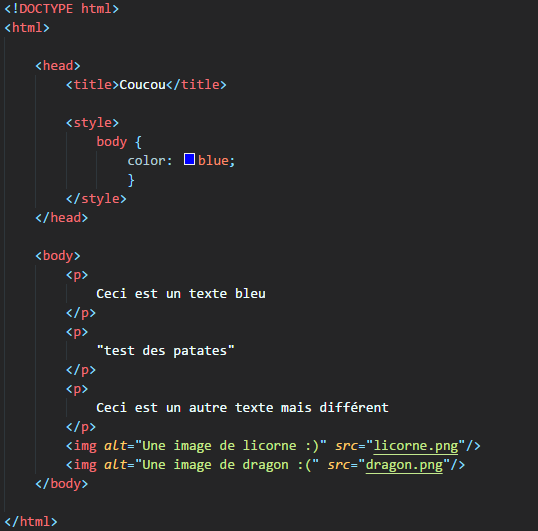
\includegraphics[height=1\textwidth]{html3.png}
\caption{\label{fig:html2}Fichier HTML avec plusieurs sur lesquelles ont été réalisé et approfondis les tests}
\end{figure}

\begin{figure}[ht]
\centering
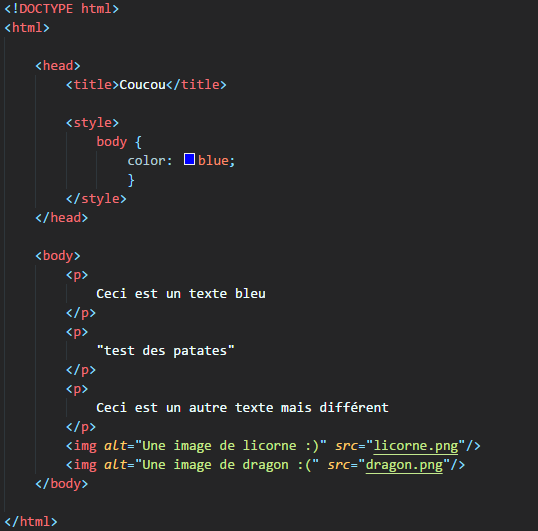
\includegraphics[height=1\textwidth]{html3.png}
\caption{\label{fig:html3}Fichier HTML avec plusieurs sur lesquelles ont été réalisé et approfondis les tests}
\end{figure}